\chapter*{Popis a rozbor problému}

\par Realistické zobrazení zemského povrchu představuje vzhledem ke svému nepravidelnému tvaru poměrně komplikovaný proces. Modelovat a popsat takový 3D model je obtížné i vzhledem ke kartografickým zásadám a estetickým požadavkům, případně i k požadavku matematicky snadného definování. V současné době je snaha vytvářet za použití výpočetní techniky tzv. \emph{digitální modely terénu} (dále jen DMT), které kromě reprezentace terénu ve 3D prostoru zahrnují řadu dalších kartografických technik, pomocí kterých je možné vyjádřit jeho charakter (Bayer 2008). Jedná se především o izočáry, stínování terénu, znázorňování sklonů, hypsometrie apod.
\par Obecně se v souvislosti s digitálním modelem terénu rozlišují dva základní pojmy, a to \textbf{DMT} a \textbf{DMP}. DMT je digitální reprezentace zemského povrchu bez zásahu lidské činnosti (tzn. bez budov), ale i přírodní sféry. V literatuře se také zmiňuje pojmem \textbf{DMR} (digitální model reliéfu), jehož význam je totožný jako pro pojem DMR.  DMP (digitální model povrchu) reprezentuje zemský povrch včetně střech budov, korun stromů a dalších umělých i přírodních objektů na zemském povrchu. Dále se může v literatuře vyskytnout termín \textbf{DVM}, což je zkratka pro digitální výškový model, který pracuje výhradně s nadmořskými výškami bodů. Jak poznamenává Brůha (2016), v zahraniční literatuře se vyskytuje pro označení digitálních modelů terénu termín \textbf{DEM}, který může vyjadřovat jak digitální výškový model, tak i digitální model povrchu nebo i reliéfu.
\par Digitální reprezentace terénu nachází uplatnění při plánování výstavby a infrastruktury, ale například i k výpočtu \textbf{sklonu} (anglicky \emph{slope}) a \textbf{orientaci svahu} (anglicky \emph{aspect}), což je užitečné pro vyhodnocení hrozby přírodních rizik, jako jsou sesuvy půdy, eroze, či pády laviny. Dále se využívá v geovědních oborech pro operaci s obrazovými daty, ve vojenství, lesnictví, počítačové grafice a mnoha dalších výzkumných i komerčních sférách.
\par V praxi jsou nejčastěji používány 3 typy DMT:
\begin{itemize}
    \item trojúhelníkový model terénu (polyedrický model),
    \item rastrový model terénu,
    \item plátový model terénu.
\end{itemize}
\par Cílem této úlohy je vytvořit model trojúhelníkový pomocí 2D \emph{Delaunay triangulace}, a následně na něm provést analýzu výškopisu, sklonu a expozice.

\section*{Konstrukce DMT}
\par Trojúhelníkový model terénu je založen na reprezentaci sítí trojúhelníkových ploch (obr. 1). Síť trojúhelníků (označovaná jako \textbf{TIN} – \emph{triangulated irregular network}) je vytvořena za použití triangulačního algoritmu, který prokládá trojicí vrcholů rovinu v $\mathbb{R}^3$, čímž vzniká nepravidelný mnohostěn přimykající se k terénu (Brůha 2016). V rámci trojúhelníku je pak prováděna lineární, nebo jiné typy interpolací pro další analýzy.

\begin{figure}[H]
\centering
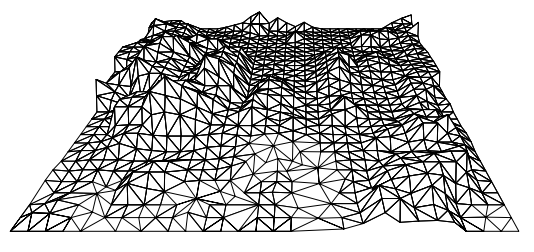
\includegraphics[width=10cm]{images/tin.png} 
    \caption{Ukážka trojúhelníkového modelu terénu (převzato z de Berg a kol. (2008, s. 191)).}
\end{figure}


\par Vhodný triangulační algoritmus musí splňovat několik kritérií. Zásadní kritérium pro DMT je tvar trojúhelníků v TIN, které by se měli co nejvíce podobat rovnostranným trojúhelníkům tak, aby se výsledná síť co nejvíce přimykala k terénu. Tohoto požadavku lze dosáhnout maximalizací minimálního úhlu v trojúhelnících (koncept využívaný právě v Delaunayho triangulaci, Bayer 2023). Další kritéria můžou představovat např. schopnost triangulovat nekonvexní oblasti, oblasti obsahující díry, nebo schopnost vkládat povinné hrany trojúhelníků, čímž se ovlivní tvar terénu. 
\bigbreak

\subsection*{Delaunayho triangulace}
\par \emph{Delaunayho triangulace} (dále jen $\mathcal{DT}$) je jedna z nejčastěji používaných triangulací, v oblastí GIS představuje standard. Lze ji tvořit jak ve 2D, tak ve 3D prostoru. Má následující vlastnosti:

\begin{itemize}
  \item Uvnitř kružnice opsané libovolnému trojúhelníku \emph{t} v $\mathcal{DT}$ neleží žádný jiný bod množiny P. 
  \item $\mathcal{DT}$ maximalizuje minimální úhel v $\forall$\emph{t}, avšak $\mathcal{DT}$ neminimalizuje maximální úhel v \emph{t}.
  \item $\mathcal{DT}$ je lokálně optimální i globálně optimální vůči kritériu minimálního úhlu.
  \item $\mathcal{DT}$ je jednoznačná, pokud žádné čtyři body neleží na kružnici. 
\end{itemize}

\par Výsledné trojúhelníky $\mathcal{DT}$ se pak vizuálně podobají rovnostranným trojúhelníkům (obr. 2).
\begin{figure}[H]
\centering
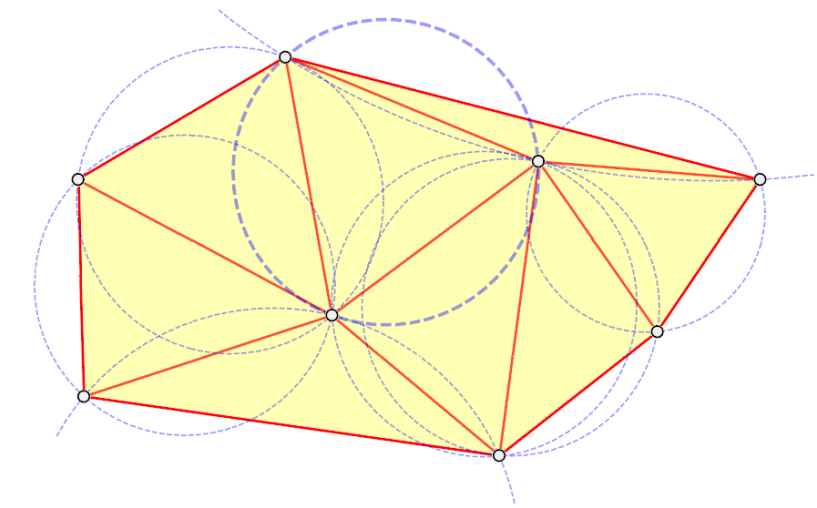
\includegraphics[width=10cm]{images/dt.png} 
    \caption{Ukázka $\mathcal{DT}$ (převzato z Bayer 2023).}
\end{figure}

\par Metod přímé konstrukce $\mathcal{DT}$ existuje několik, pro jednoduchost bude v této úloze implementována varianta inkrementální konstrukce s časovou složitostí $O(n^3)$. Tato metoda je založena na postupném přidávání bodů do již vytvořené $\mathcal{DT}$. 

\par Je daná \emph {množina P} tvořená body $\{p_1, \dots, p_n\}$, kde každý bod $p_i = \{x_i, y_i, z_i\}$. Algoritmus prochází každý bod $p_i \in P$ a hledá k němu nejbližší bod takový, jehož euklidovská vzdálenost k němu je nejmenší. Nalezne-li se tento bod, vznikne první (orientovaná) Delaunayovská hrana \emph{e} ve vznikajícím trojúhelníku, která je tvořená body ($p_1$,$p_2$). K hraně \emph{e} se následně bude hledat třetí bod $\overline{p}$ do trojúhelníku, který:

\begin{itemize}
    \item leží v levé polorovině od orientované hrany \emph{e},
    \item maximalizuje vnitřní úhel $\angle (p_1,p,p_2)$:
\end{itemize}

\begin{equation*}
\overline{p} = arg\underset{\forall p_i \in \sigma L (e)}{\max}\angle (p_1,p,p_2),
\end{equation*}

\par kde $p_i \in \sigma_l (e)$. Pokud takový bod $\overline{p}$ neexistuje, změní se orientace hrany $e$ a hledání bodu $\overline{p}$ se opakuje stejným způsobem.
\par Do $\mathcal{DT}$ je přidán seznam hran trojúhelníku $\triangle (p_1, p_2, \overline{p})$:

\begin{equation*}
e_1 = (p_2, \overline{p}), \quad e_2 = (\overline{p}, p_1),
\end{equation*}

\par pokud splní podmínku, že opačně orientované hrany

\begin{equation*}
e_1' = (\overline{p}, p_2), \quad e_2' = (p_1, \overline{p}),
\end{equation*}

\par nejsou v \emph{AEL} (Active Edges List) – v aktivním seznamu hran. Tato datová struktura obsahuje hrany \emph{e} takové, ke kterým se hledají body $\overline{p}$. Pokud se tento seznam vyprázdní, $\mathcal{DT}$ je vytvořena.
\bigbreak
\begin{algorithm}[H]
\caption{Pseudokód inkrementální konstrukce $\mathcal{DT}$}\label{alg:cap}
\begin{algorithmic}
\State Inicializuj $AEL = []$, $\mathcal{DT}$ = []
\State Zvol bod $p_1 \in P$ s minimální x-ovou souřadnicí
\State Najdi bod $p_2$, který má k $p_1$ nejmenší vzdálenost
\State Vytvoř hrany $e = [p_1, p_2], e' = [p_2, p_1]$
\State $AEL \gets e, AEL \gets e'$
\While {$AEL$ není prázdný}
  \State Vezmi první hranu $e$ z $AEL$
  \State Prohoď její orientaci
  \State Najdi k této hraně Delaunayovský bod $\underline{p}$
  \If{$\exists \thinspace \overline{p}$}
      \State Vytvoř zbývající hrany trojúhelníku $e_1 = (p_2, \overline{p}), e_2 = (\overline{p}, p_1)$
      \State $\mathcal{DT} \gets e'_1$, $\mathcal{DT} \gets e_2$, $\mathcal{DT} \gets e_3$
      \State Aktualizuj $AEL$ podle hran $e_2, e_3$
    \EndIf
\EndWhile
\State {\text{\textbf{vrať} $\mathcal{DT}$}}
\end{algorithmic}
\end{algorithm}
\newpage

\section*{Konstrukce vrstevnic}
\par Vrstevnice modelu byly vytvořeny lineární interpolací. Tato metoda je založená na analytické geometrii: hledá se průsečnice roviny $\mathcal{T}$ určené trojúhelníkem $t \in \mathcal{DT}$ a vodorovné roviny s výškou $h$, co se opakuje pro každý trojúhelník. Na základě podobnosti trojúhelníků můžeme nalézt souřadnice bodů $A, B$ průsečnice podle vztahů:
\begin{equation*}
\begin{split}
    x_a & = \frac{x_3-x_1}{z_3-z_1}(z-z_1)+x_1,\\[10pt]
    y_a & = \frac{y_3-y_1}{z_3-z_1}(z-z_1)+y_1,
\end{split}
\quad \quad \quad
\begin{split}
    x_b & = \frac{x_2-x_1}{z_2-z_1}(z-z_1)+x_1,\\[10pt]
    y_b & = \frac{y_2-y_1}{z_2-z_1}(z-z_1)+y_1.
\end{split}
\end{equation*}
\par Ve vlastní implementaci je také ověřeno, zda rovina $\rho$ protíná hranu $(p_i, p_{i+1})$ trojúhelníku pomocí vztahu:
\begin{equation*}
    \Delta z_i\Delta z_{i+1} < 0,
\end{equation*}
\par kde $\Delta z_i = z_i - z, \: \: \Delta z_{i+1} = z_{i+1} - z$.
\bigbreak
\section*{Analýza sklonu terénu}
\par Pro účely analýzy hydrologických poměrů, sesuvů, návrhy komunikací, stavebních objektů atd. je potřebné získat informace o sklonu terénu na zájmovém území. V trojúhelníkovém modelu DMT je výpočet sklonu proveden nad každým trojúhelníkem pomocí gradientu (obr. 3). 
\par Obecná rovnice roviny $\rho$ má tvar:
\begin{equation*}
    \rho : ax + by + cz + d = 0,
\end{equation*}
\par gradient $\nabla f(x_0, y_0, z_0)$ funkce $f(x, y, z)$ v bodě $p = [x_0, y_0, z_0]$ pak určuje vztah: \vspace{10pt}
\begin{equation*}
    \nabla f (x_0, y_0, z_0) = \left(\frac{\partial f}{\partial x}(x_0), \frac{\partial f}{\partial y}(y_0), \frac{\partial f}{\partial z}(z_0)\right) = (a, b, c)
\end{equation*}
\par Mějme vodorovnou rovinu $\pi$. Roviny $\rho$ a $\pi$ mají normálové vektory $n_1, n_2$, přičemž pro rovinu $\pi$ uvažujeme s jednotkovým vektorem:
\begin{equation*}
    n_1 = (a, b, c), \quad n_2 = (0, 0, 1),
\end{equation*}
\par odchylku $\varphi$ rovin $\rho$ a $\pi$ – hledaný sklon pak určíme ze vztahu: \vspace{10pt}
\begin{equation*}
    \varphi = \arccos{\frac{n_1 \cdot n_2}{\|n_1\| \|n_2\|}} = \arccos{\frac{c}{\|n_1\|}}.
\end{equation*}
\begin{figure}[H]
\centering
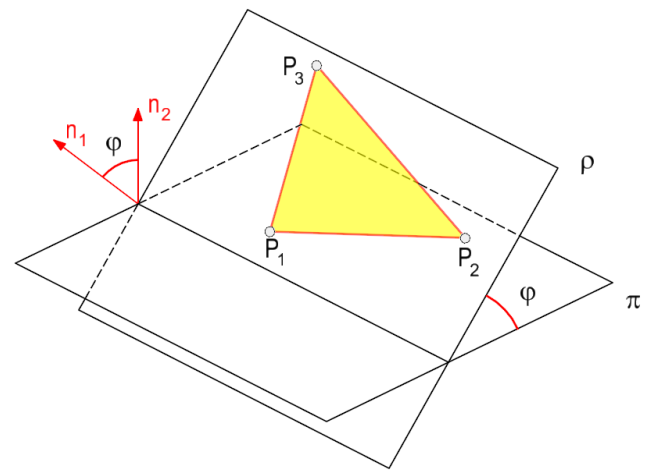
\includegraphics[width=9cm]{images/slope.png} 
    \caption{Vizualizace výpočtu sklonu trojúhelníka (převzato z Bayer 2023).}
\end{figure}

\section*{Analýza expozice terénu}
\par Expozice, resp. orientace terénu je definovaná jako azimut průmětu gradientu $\nabla \rho$ do roviny $x, y$, čímž vznikne vektor $\Vec{v}$ s nulovou složkou $z$ (obr. 4):\vspace{10pt}
\begin{equation*}
    \Vec{v} = \left(\frac{\partial \rho}{\partial x}(x_0), \frac{\partial \rho}{\partial y}(y_0), 0\right) = (a, b, 0).
\end{equation*}
\par Azimut $A$ vektoru $\Vec{v}$ je pak měřen od osy $y$ dle vztahu:
\begin{equation*}
    A = \arctan{\left(\frac{a}{b}\right)},
\end{equation*}
\par ve vlastní implementaci jsou však pro účely správné vizualizace potřebné dodatečné korekce: v prostředí $Canvas$ frameworku QT je kladný směr osy $y$ dolu (došlo tedy k prohození odčítání severního a jižního směru) a místo $\arctan$ byla využita funkce $\arctan2$.
\par Analýza expozice terénu nachází využití zejména v zemědělství, hydrologii a stavebnictví.
\begin{figure}[H]
\centering
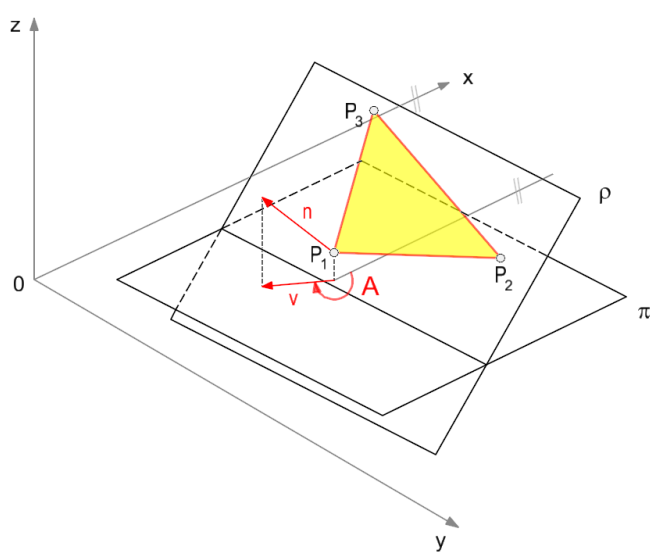
\includegraphics[width=9cm]{images/aspect.png} 
    \caption{Vizualizace výpočtu orientace trojúhelníka (převzato z Bayer 2023).}
\end{figure}